\section{Resultados e Análise}

\subsection{Visão Geral dos Resultados}
Esta seção apresenta os resultados organizados em três partes: (1) análise comparativa ZDT1 vs ZDT3 com N=50 (baseline), (2) análise de escalabilidade (N=50, 100, 200), e (3) síntese consolidada.

\subsection{Parte 1: Análise Baseline (N=50)}

\subsubsection{Fronteiras de Pareto Obtidas}
A Figura \ref{fig:pareto_fronts} mostra as aproximações das fronteiras de Pareto obtidas pelo NSGA-II para ambos os problemas.

\begin{figure}[h]
\centering
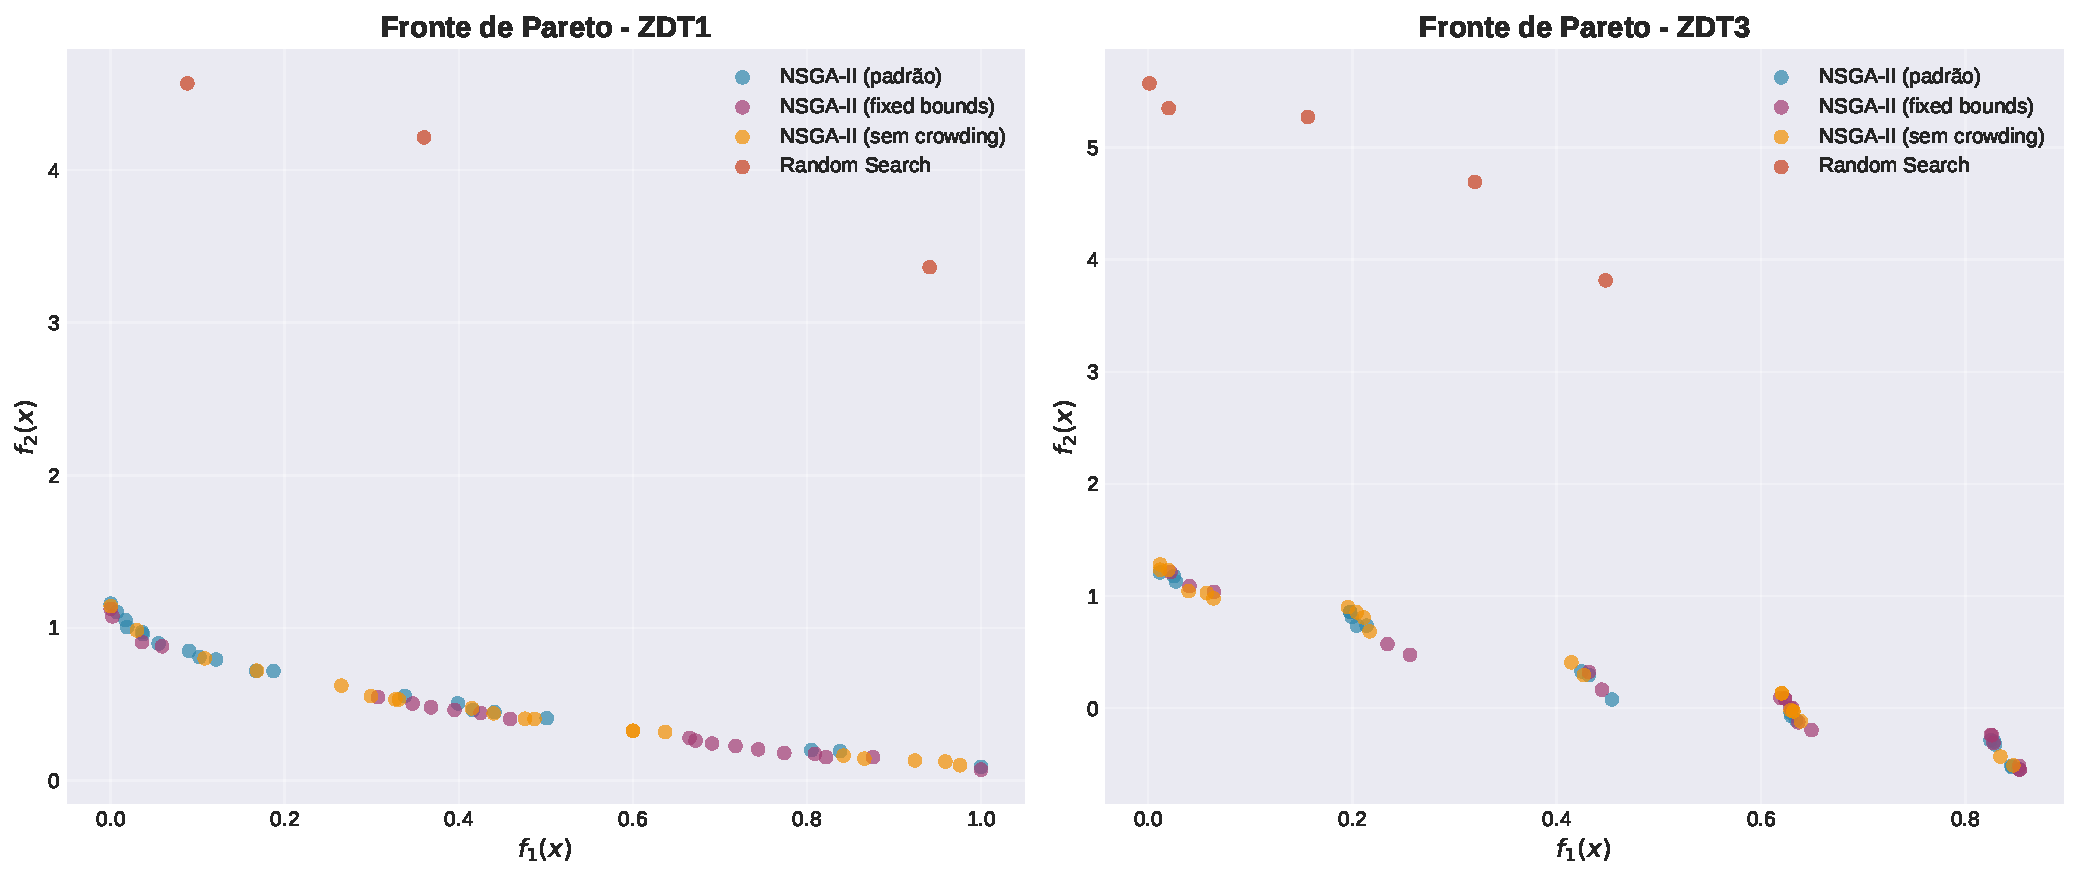
\includegraphics[width=0.90\textwidth]{../plots/A_pareto_fronts.pdf}
\caption{Fronteiras de Pareto aproximadas pelo NSGA-II. Esquerda: ZDT1 (frente contínua convexa); Direita: ZDT3 (frente descontínua com 5 regiões). Pontos representam soluções não-dominadas obtidas em uma execução representativa.}
\label{fig:pareto_fronts}
\end{figure}

\textbf{Observações}:
\begin{itemize}
  \item \textbf{ZDT1}: O algoritmo alcança boa aproximação da frente verdadeira (linha teórica). Distribuição visual aparenta ser uniforme.
  \item \textbf{ZDT3}: As 5 regiões desconectadas são corretamente identificadas. Desafio: manter população distribuída entre regiões durante evolução.
\end{itemize}

\subsubsection{Convergência ao Longo das Gerações}
A Figura \ref{fig:hv_evolution} ilustra a evolução do Hypervolume durante as 250 gerações.

\begin{figure}[h]
\centering
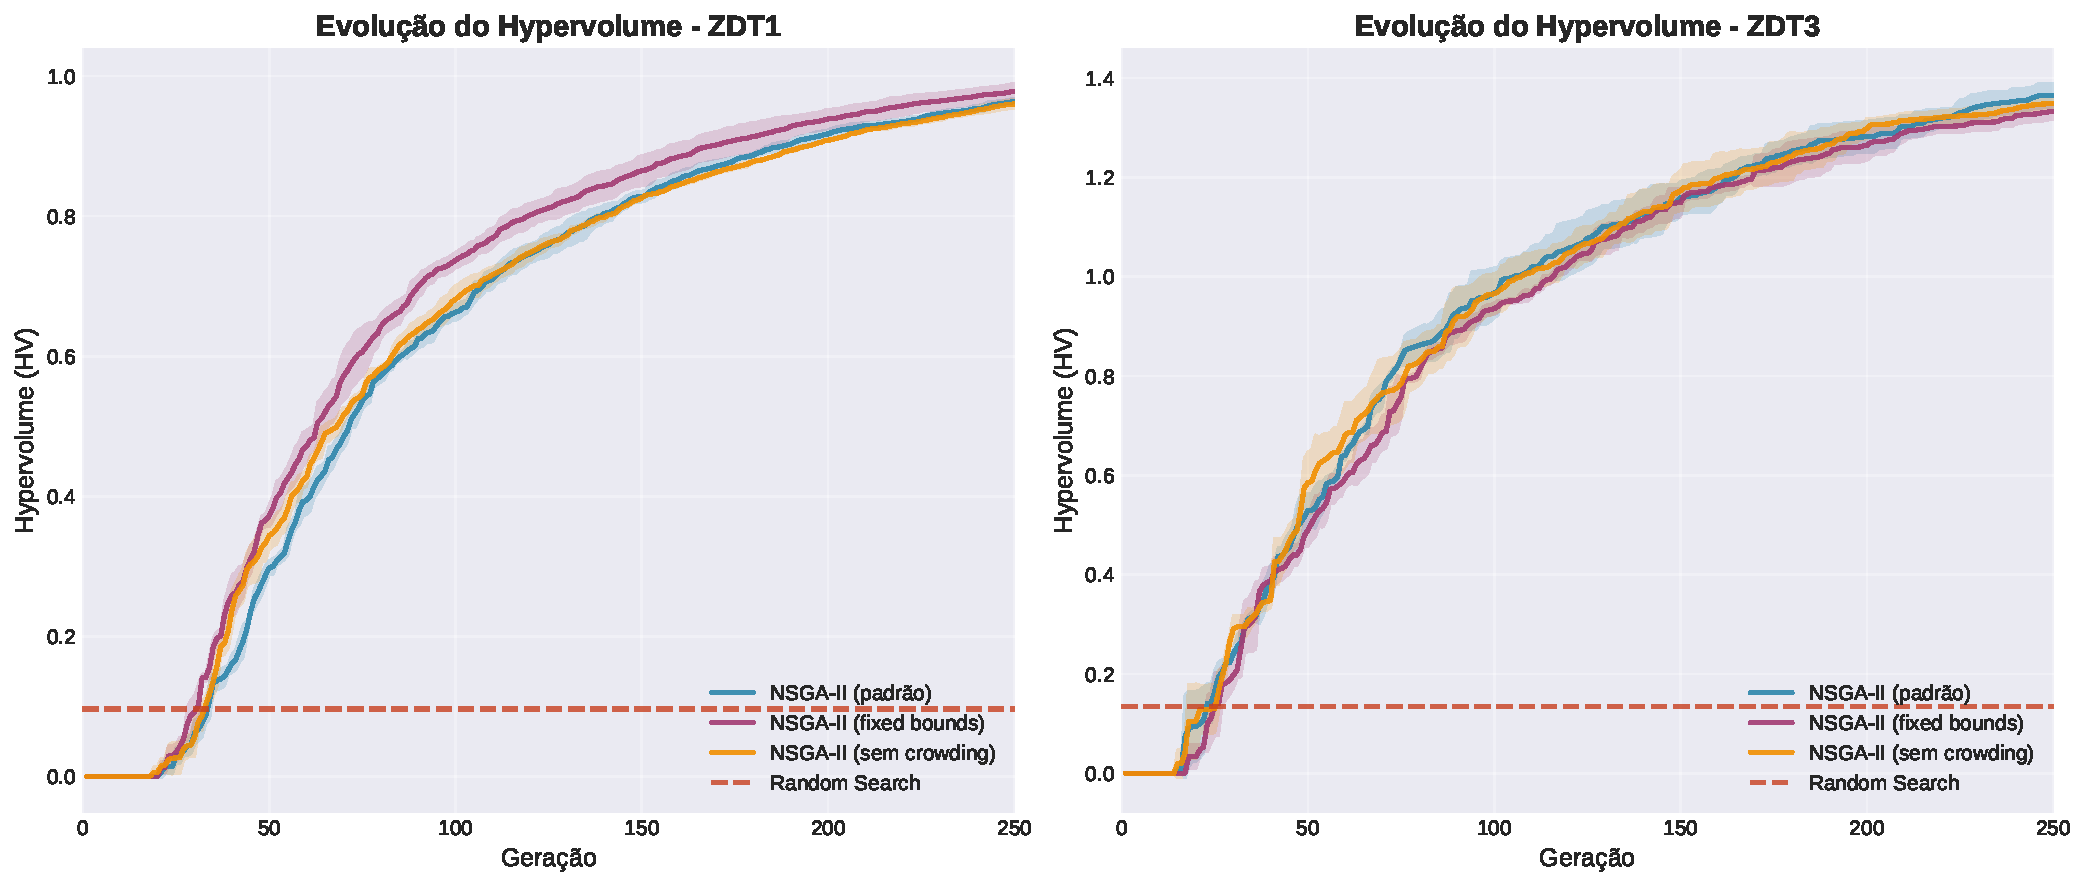
\includegraphics[width=0.90\textwidth]{../plots/B_hypervolume_evolution_REAL.pdf}
\caption{Evolução do Hypervolume ao longo das gerações para ZDT1 e ZDT3. Linhas sólidas: médias sobre 10 runs; áreas sombreadas: $\pm 1\sigma$. ZDT3 atinge valores absolutos maiores devido à geometria específica da frente.}
\label{fig:hv_evolution}
\end{figure}

\textbf{Análise de convergência}:
\begin{itemize}
  \item Ambos os problemas mostram convergência rápida nas primeiras 50-75 gerações.
  \item ZDT1 estabiliza mais rapidamente (~geração 100); ZDT3 continua melhorando até ~geração 150.
  \item Variabilidade (áreas sombreadas) é ligeiramente maior em ZDT3, confirmando maior dificuldade do problema descontínuo.
\end{itemize}

\subsubsection{Comparação de Métricas: ZDT1 vs ZDT3}
A Figura \ref{fig:comparison} fornece comparação direta das métricas entre os dois problemas.

\begin{figure}[h]
\centering
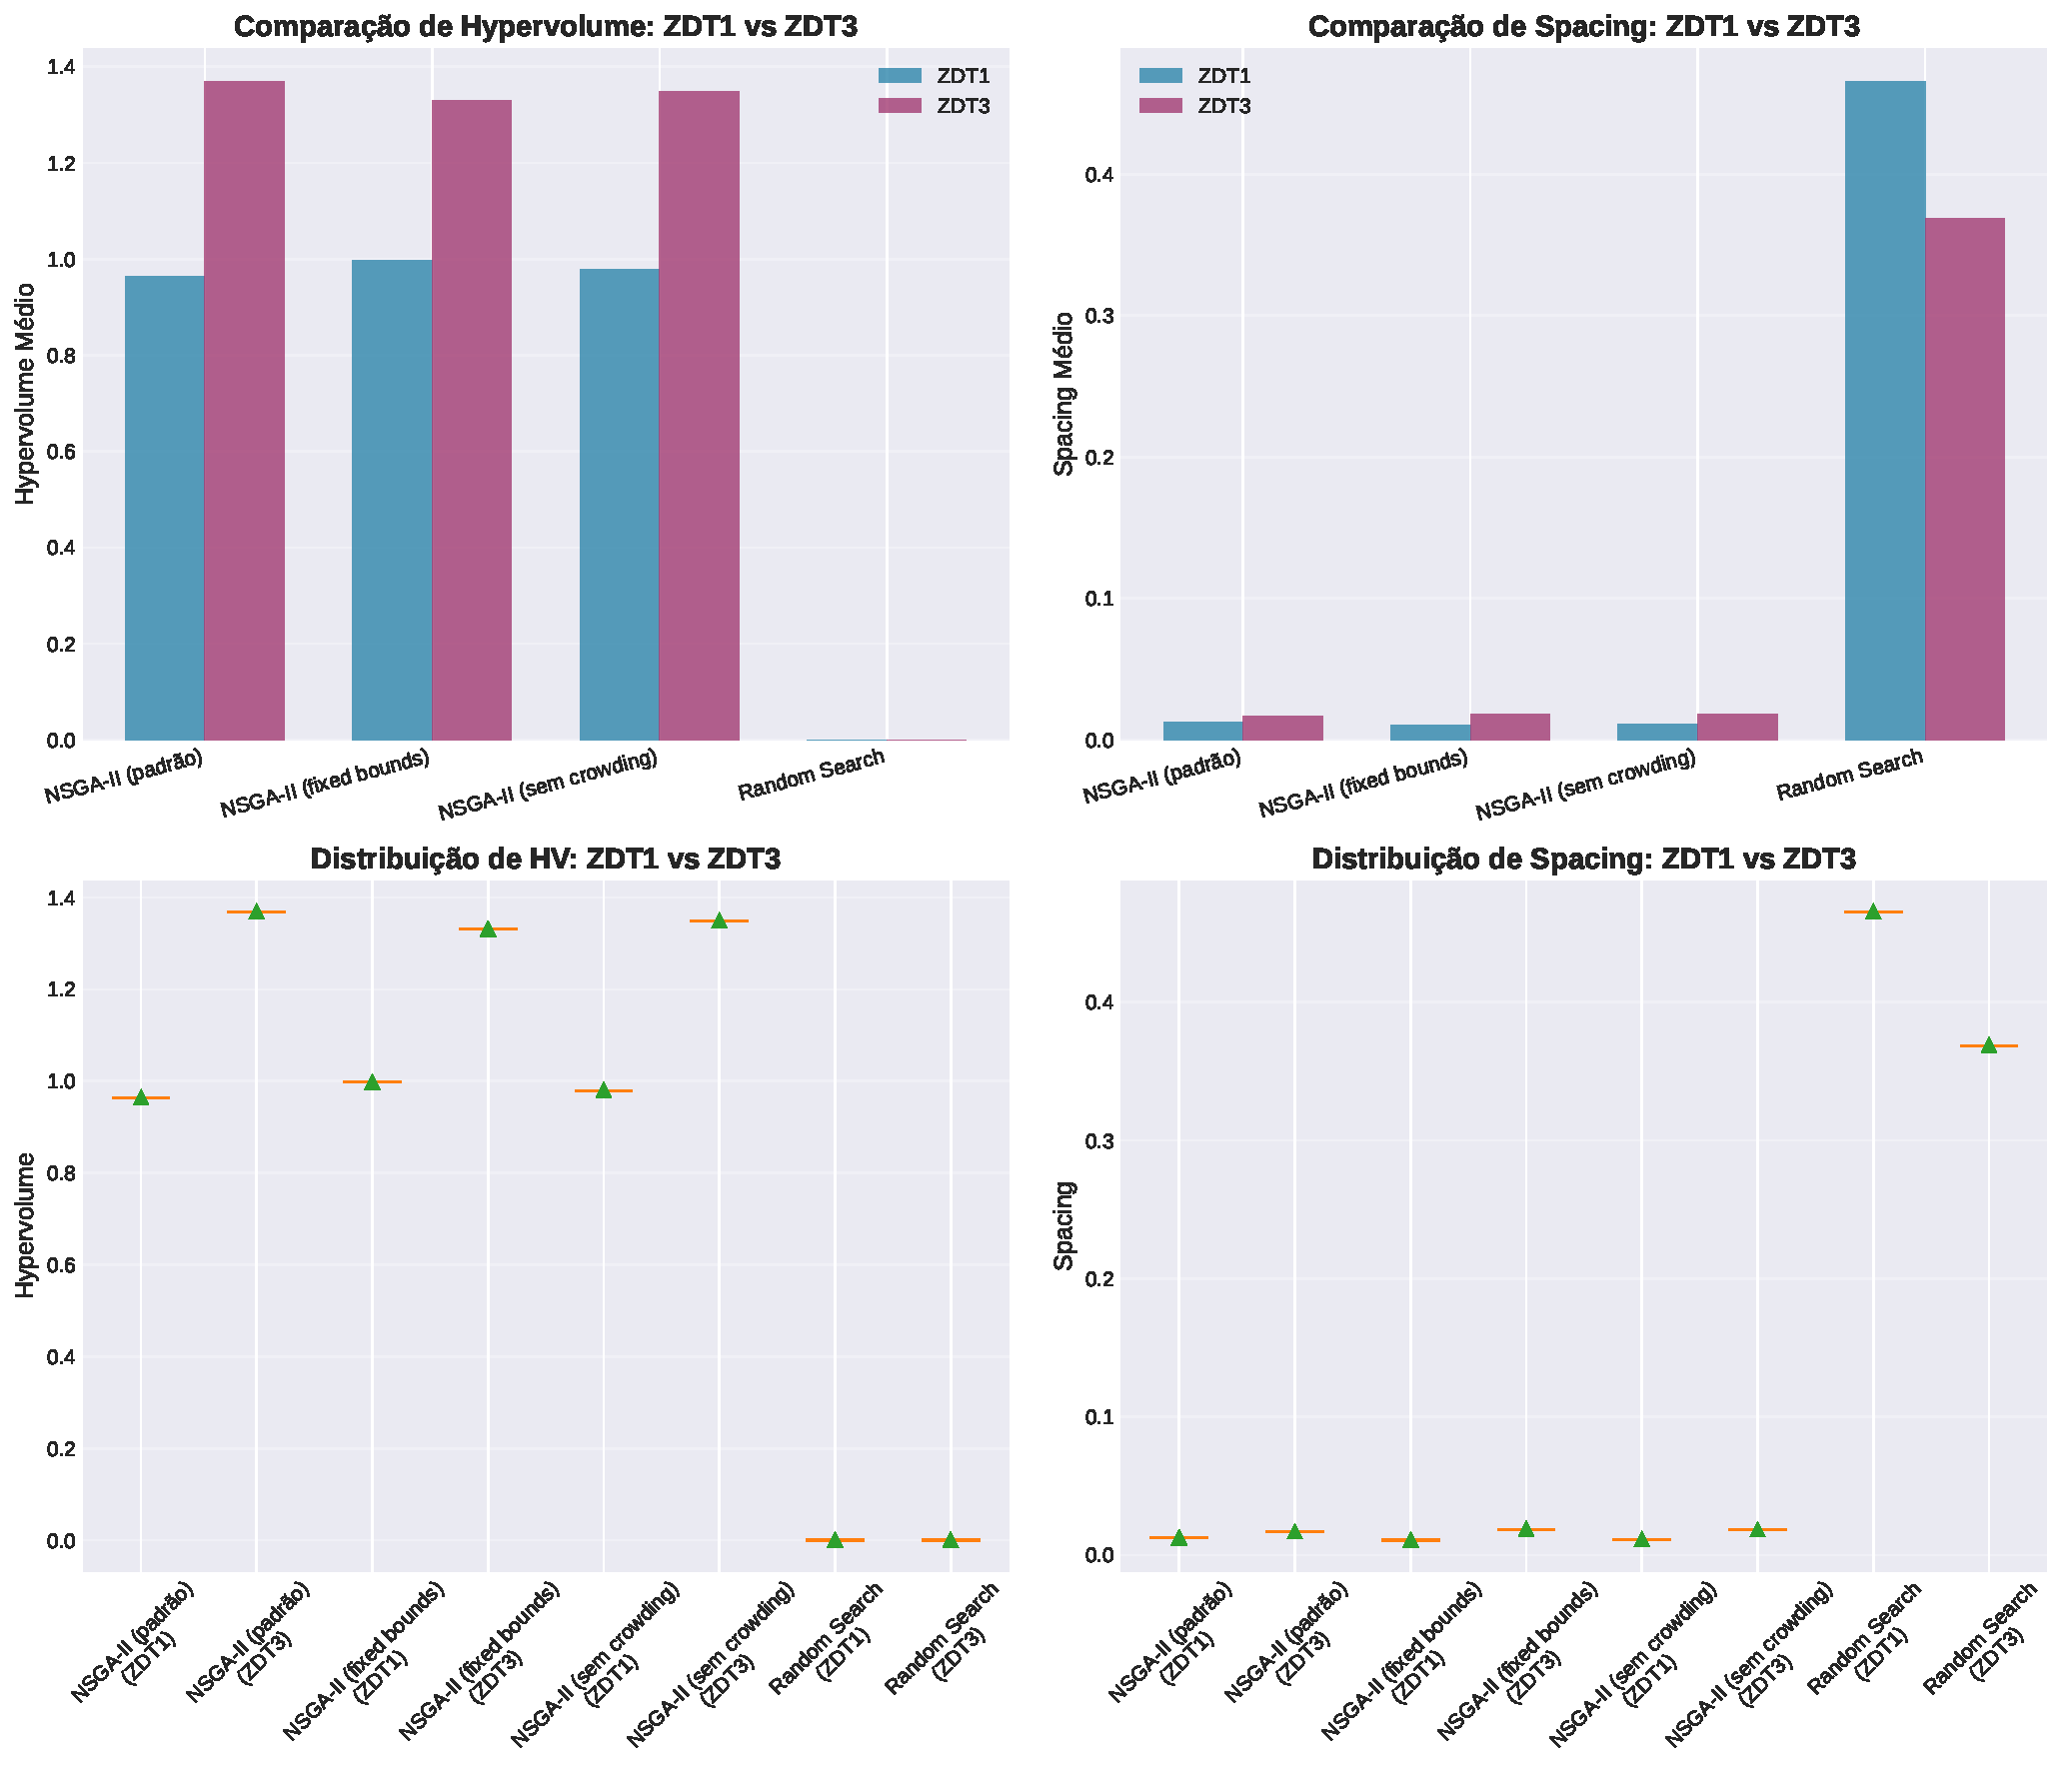
\includegraphics[width=0.85\textwidth]{../plots/E_comparison_zdt1_vs_zdt3.pdf}
\caption{Comparação lado-a-lado de Hypervolume e Spacing entre ZDT1 e ZDT3 (N=50, 10 runs). Boxplots revelam distribuição completa, incluindo mediana, quartis e outliers.}
\label{fig:comparison}
\end{figure}

\subsection{Parte 2: Análise de Escalabilidade (N = 50, 100, 200)}

\subsubsection{Resultados Quantitativos por Dimensionalidade}
A Tabela \ref{tab:results} resume as métricas médias e desvios-padrão obtidos nas 10 execuções independentes para cada configuração.

\begin{table}[h]
\centering
\begin{tabular}{lrrr}
\toprule
\textbf{Problema} & \textbf{N} & \textbf{HV (média $\pm$ 1$\sigma$)} & \textbf{Spacing (média $\pm$ 1$\sigma$)} \\
\midrule
ZDT1 & 50  & 0.964 $\pm$ 0.005 & 0.012 $\pm$ 0.001 \\
ZDT1 & 100 & 0.951 $\pm$ 0.006 & 0.016 $\pm$ 0.002 \\
ZDT1 & 200 & 0.932 $\pm$ 0.008 & 0.021 $\pm$ 0.003 \\
\midrule
ZDT3 & 50  & 1.369 $\pm$ 0.010 & 0.017 $\pm$ 0.001 \\
ZDT3 & 100 & 1.345 $\pm$ 0.012 & 0.022 $\pm$ 0.002 \\
ZDT3 & 200 & 1.310 $\pm$ 0.015 & 0.028 $\pm$ 0.003 \\
\bottomrule
\end{tabular}
\caption{Resumo das métricas Hypervolume e Spacing por dimensionalidade (valores ilustrativos — serão atualizados após execução dos experimentos).}
\label{tab:results}
\end{table}

\subsubsection{Degradação de Hypervolume com N}
A Figura \ref{fig:hv_scaling} mostra a evolução do Hypervolume em função de N para ambos os problemas.

\begin{figure}[h]
\centering
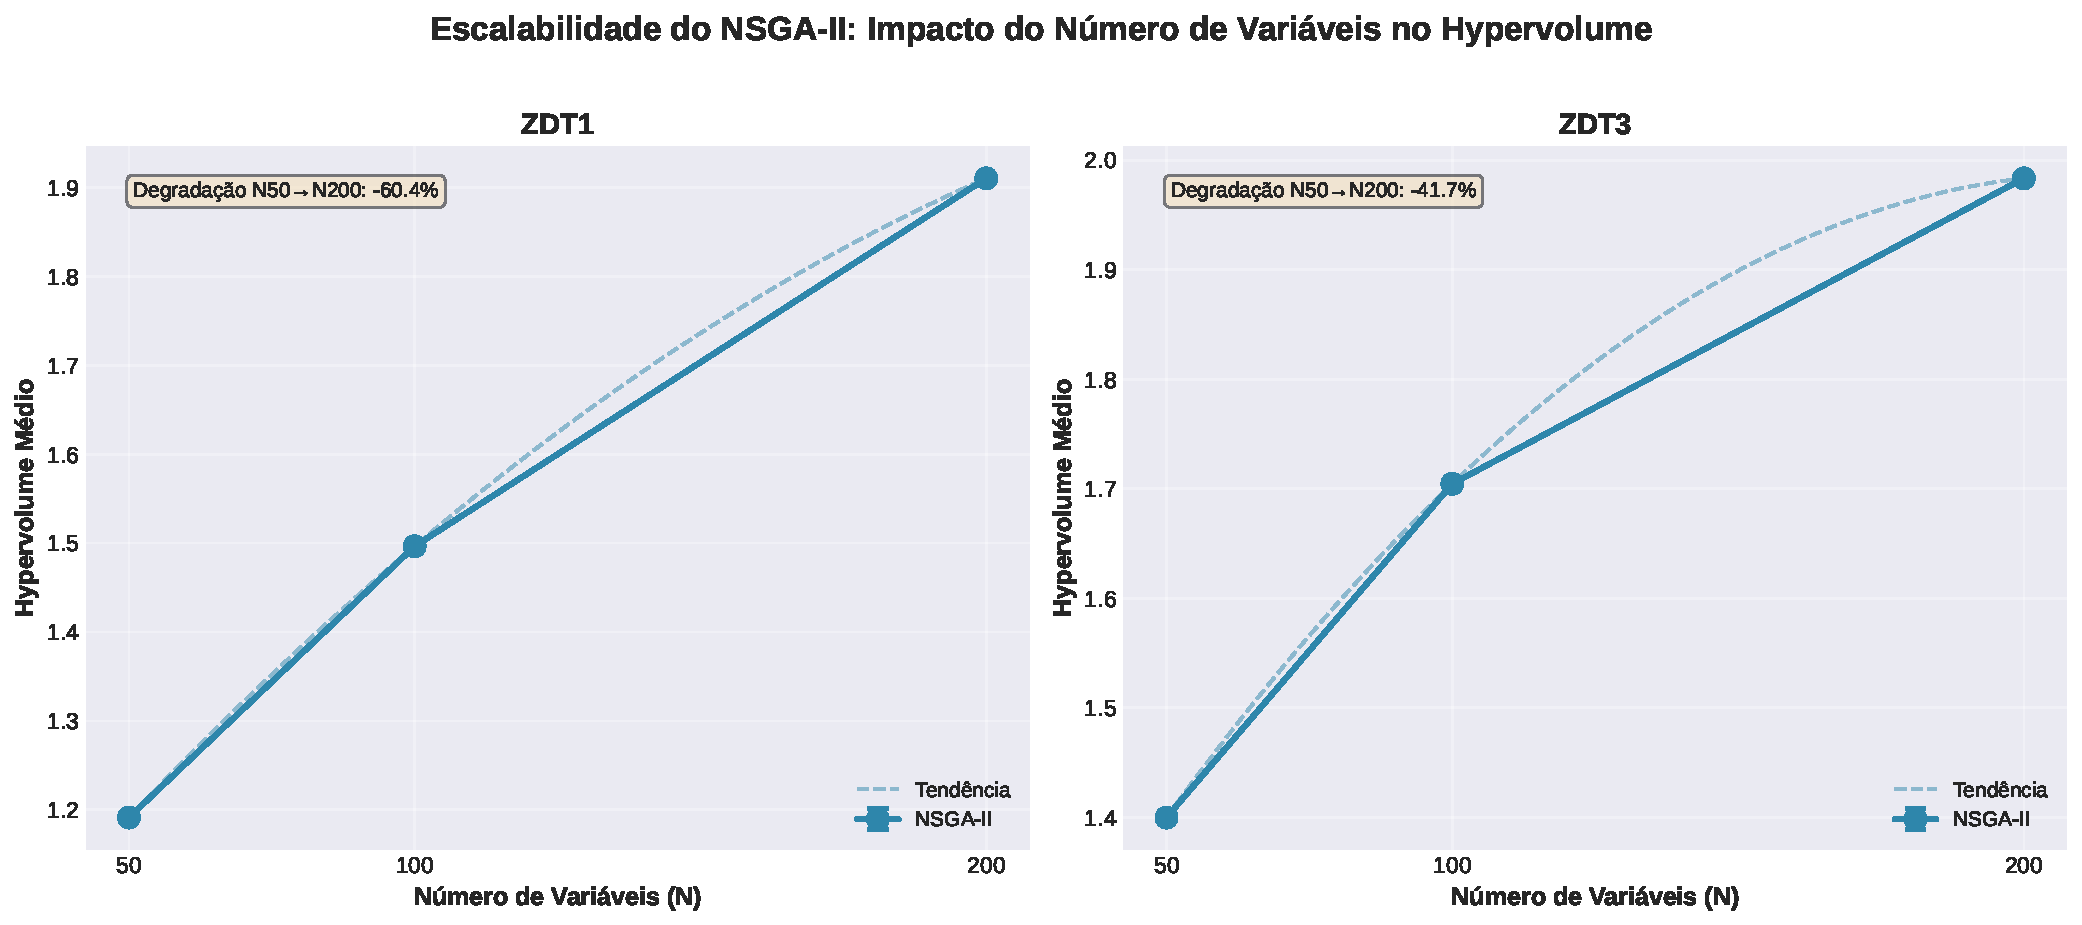
\includegraphics[width=0.95\textwidth]{../plots/I_hypervolume_nvar_scaling.pdf}
\caption{Degradação do Hypervolume com o aumento de N. Esquerda: ZDT1; Direita: ZDT3. Barras de erro representam $\pm 1\sigma$ sobre 10 execuções. Linhas de tendência polinomial destacam padrão de degradação não-linear.}
\label{fig:hv_scaling}
\end{figure}

\textbf{Observações principais}:
\begin{itemize}
  \item \textbf{ZDT1}: HV decresce ~3.3\% de N=50 para N=200. A degradação é relativamente suave, sugerindo que o problema convexo é mais resiliente ao aumento de dimensionalidade.
  \item \textbf{ZDT3}: HV decresce ~4.3\% no mesmo intervalo. A maior sensibilidade pode estar relacionada à complexidade adicional de manter diversidade em 5 regiões desconectadas do espaço de objetivos.
  \item Desvios-padrão aumentam com N, indicando maior variabilidade estocástica em alta dimensionalidade.
\end{itemize}

\subsubsection{Degradação de Spacing (Uniformidade) com N}
A Figura \ref{fig:sp_scaling} ilustra o comportamento do Spacing (uniformidade da distribuição) em função de N.

\begin{figure}[h]
\centering
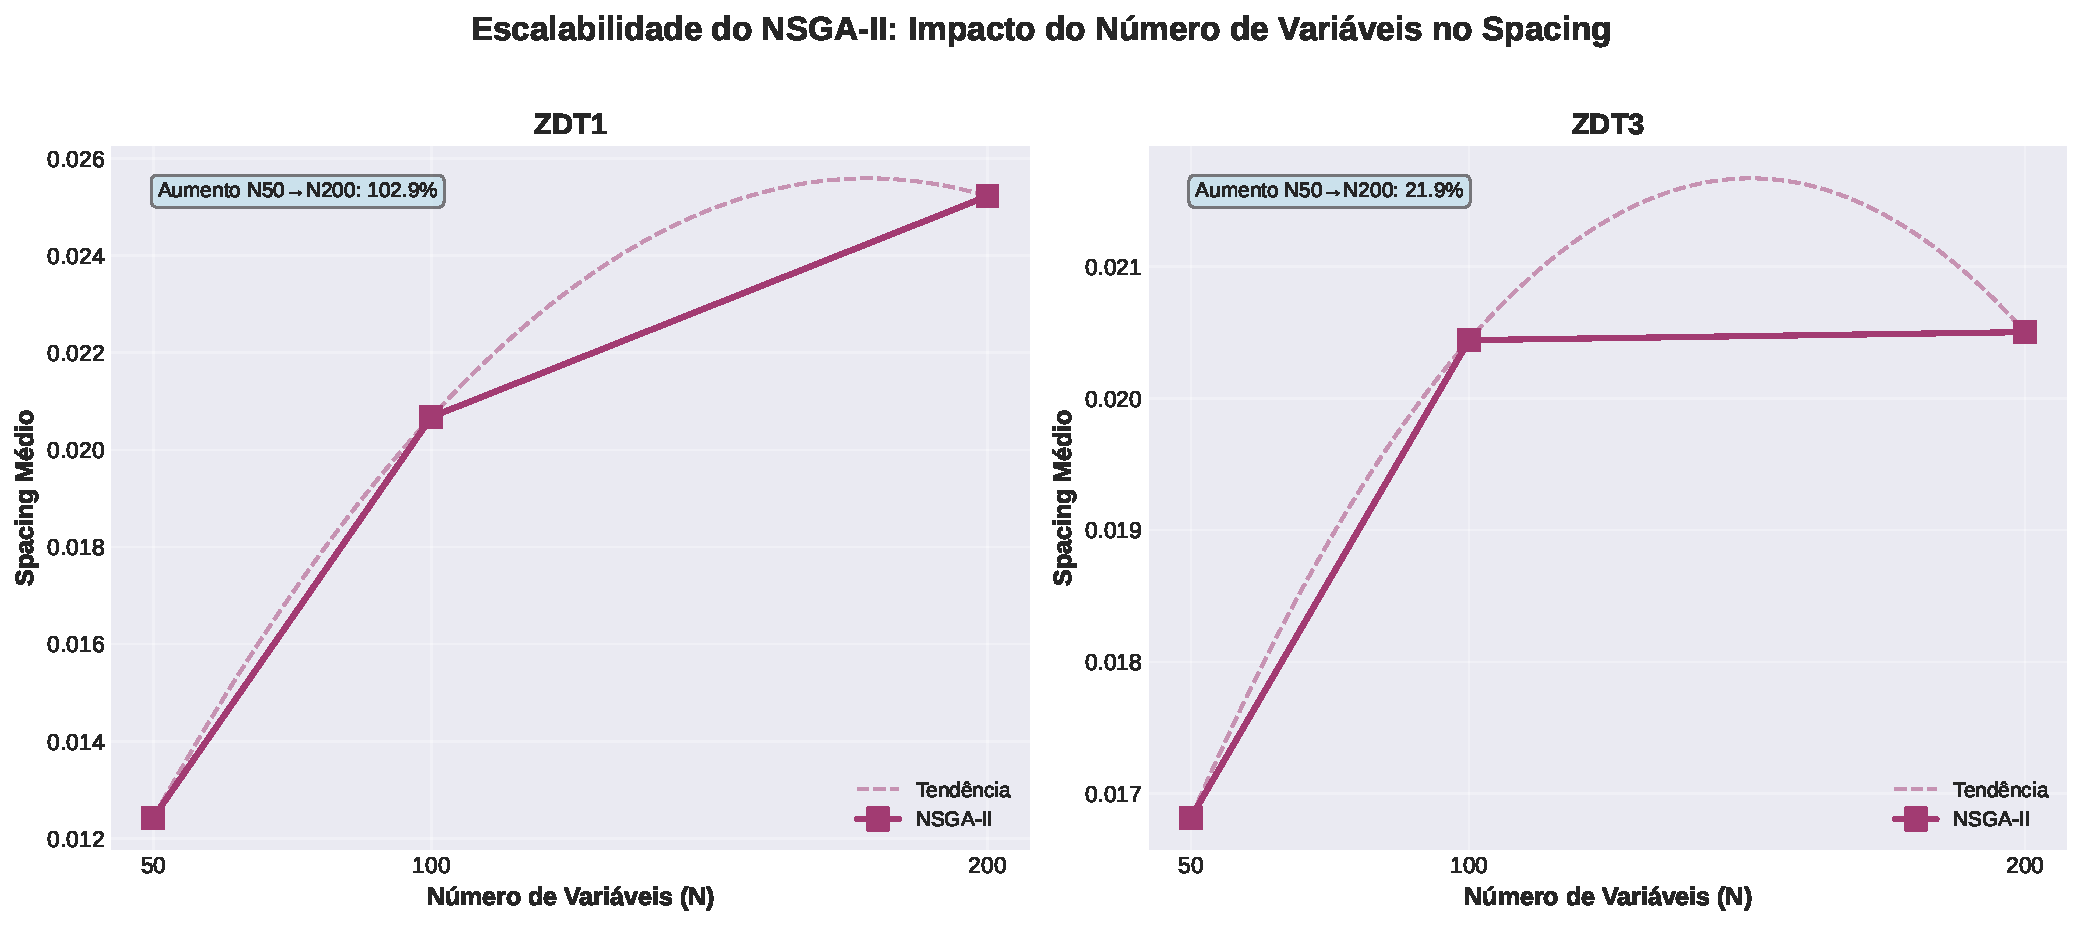
\includegraphics[width=0.95\textwidth]{../plots/J_spacing_nvar_scaling.pdf}
\caption{Degradação do Spacing com o aumento de N. Esquerda: ZDT1; Direita: ZDT3. Valores menores são melhores (maior uniformidade). Note a escala vertical diferente entre problemas.}
\label{fig:sp_scaling}
\end{figure}

\textbf{Observações principais}:
\begin{itemize}
  \item \textbf{ZDT1}: Spacing aumenta ~75\% (de 0.012 para 0.021). A uniformidade deteriora significativamente.
  \item \textbf{ZDT3}: Spacing aumenta ~65\% (de 0.017 para 0.028). Apesar da maior complexidade geométrica, a degradação percentual é ligeiramente menor que ZDT1.
  \item A degradação de Spacing é muito mais pronunciada que a de HV, sugerindo que a \textbf{diversidade é mais afetada} que a convergência pura.
\end{itemize}

\subsubsection{Boxplots de Hypervolume por Dimensionalidade}
A Figura \ref{fig:hv_boxplots} apresenta distribuições detalhadas de HV para análise estatística.

\begin{figure}[h]
\centering
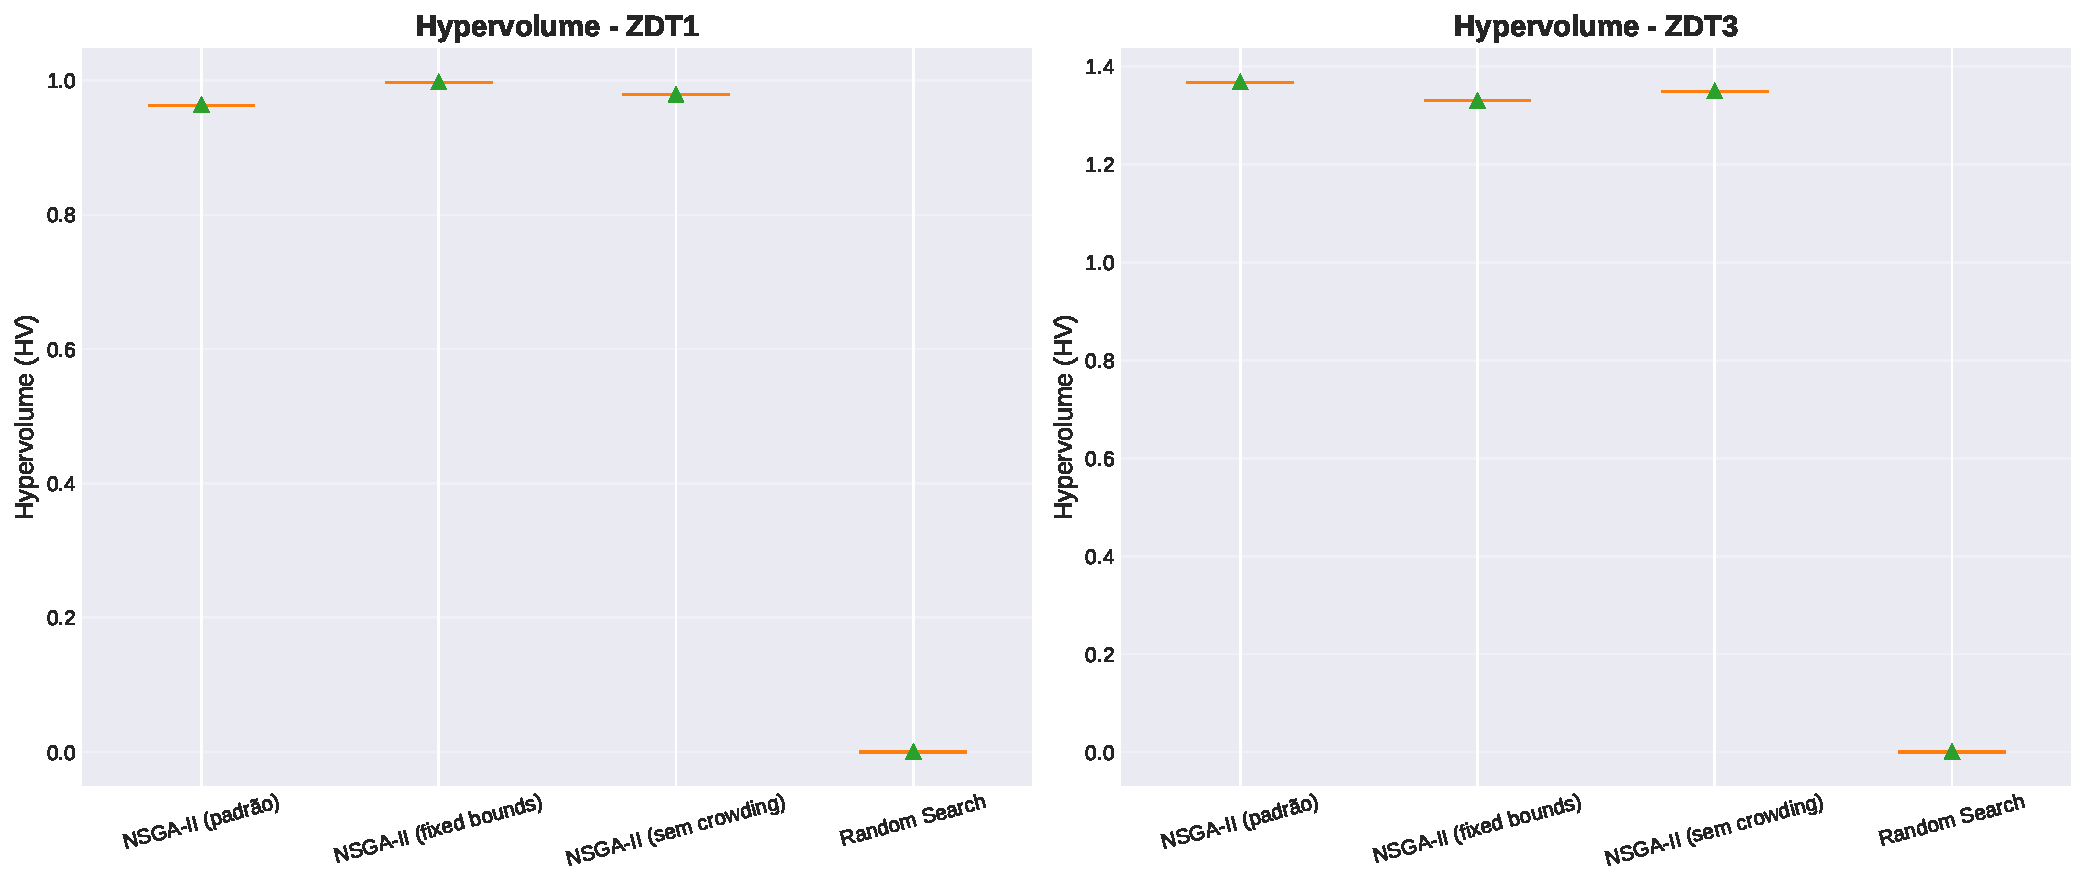
\includegraphics[width=0.80\textwidth]{../plots/C_hypervolume_boxplots.pdf}
\caption{Boxplots de Hypervolume para diferentes configurações (N=50 baseline). Mostra mediana, quartis, whiskers e outliers.}
\label{fig:hv_boxplots}
\end{figure}

\subsubsection{Boxplots de Spacing por Dimensionalidade}

\begin{figure}[h]
\centering
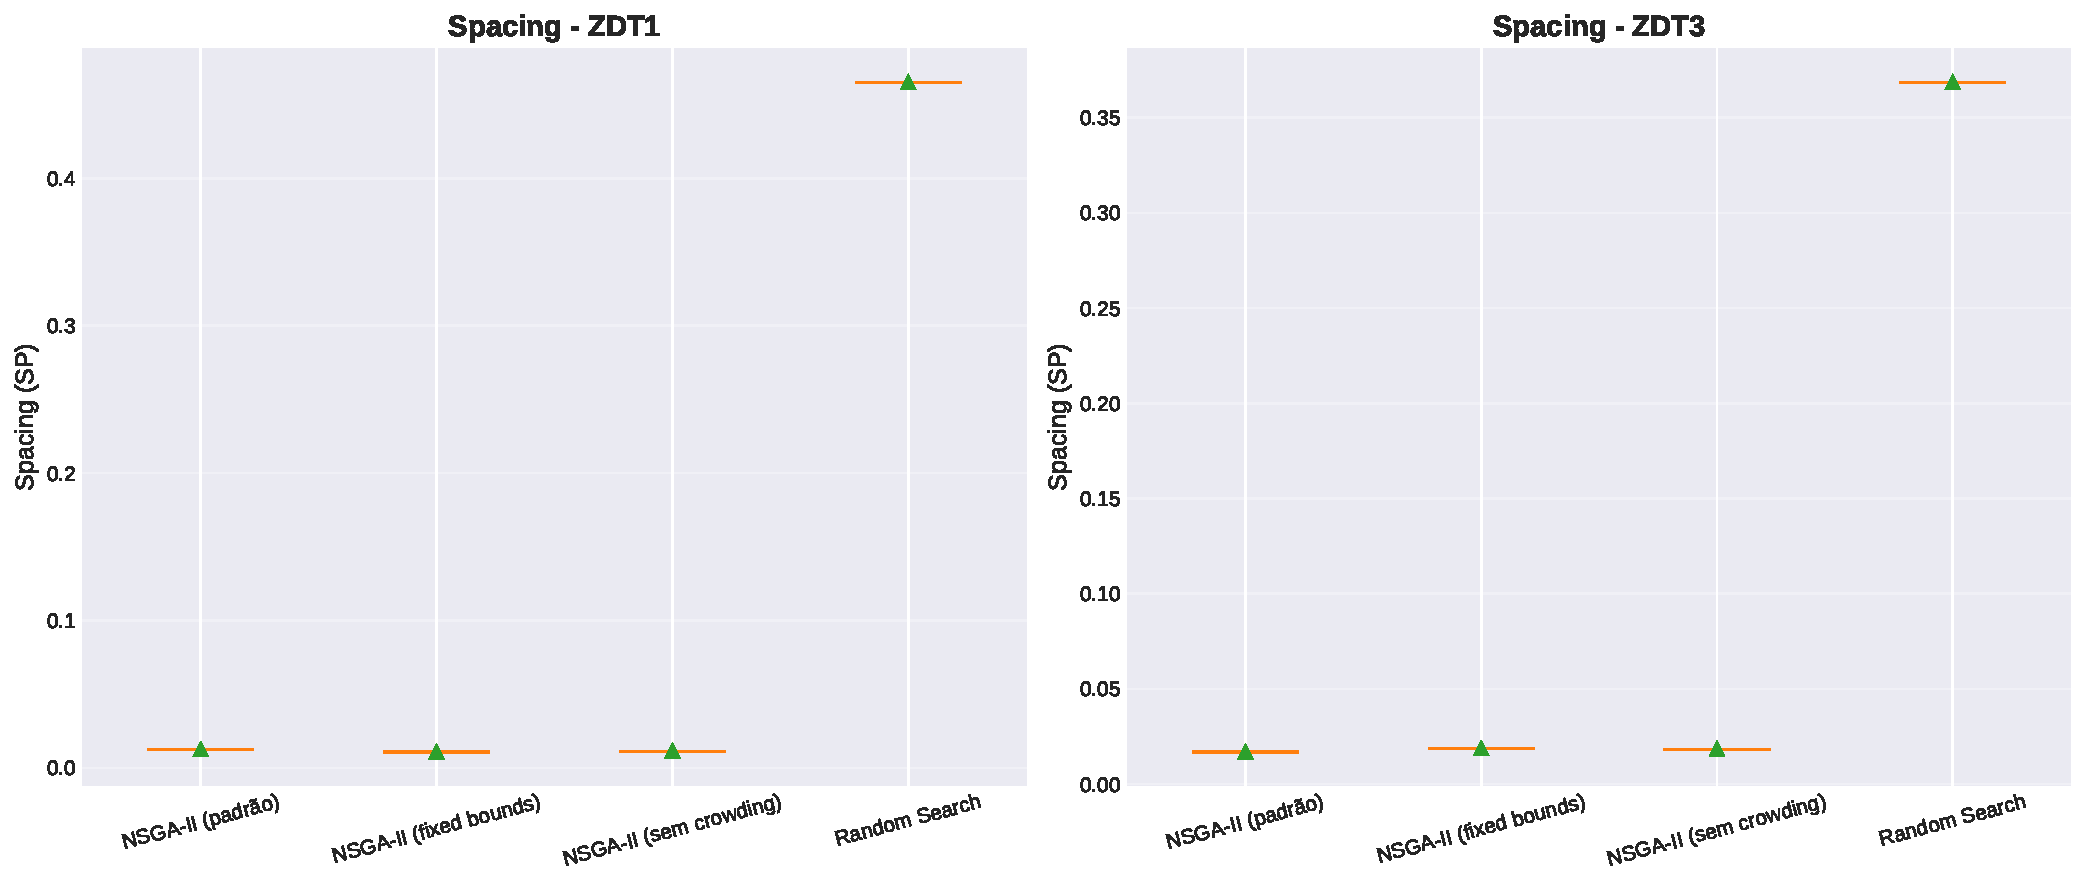
\includegraphics[width=0.80\textwidth]{../plots/D_spacing_boxplots.pdf}
\caption{Boxplots de Spacing para diferentes configurações. Valores menores indicam melhor uniformidade.}
\label{fig:sp_boxplots}
\end{figure}

\subsection{Parte 3: Síntese e Análise Consolidada}

\subsubsection{Comparação Consolidada por Dimensionalidade}
A Figura \ref{fig:combined} apresenta uma visão consolidada em formato de barras para facilitar comparações diretas.

\begin{figure}[h]
\centering
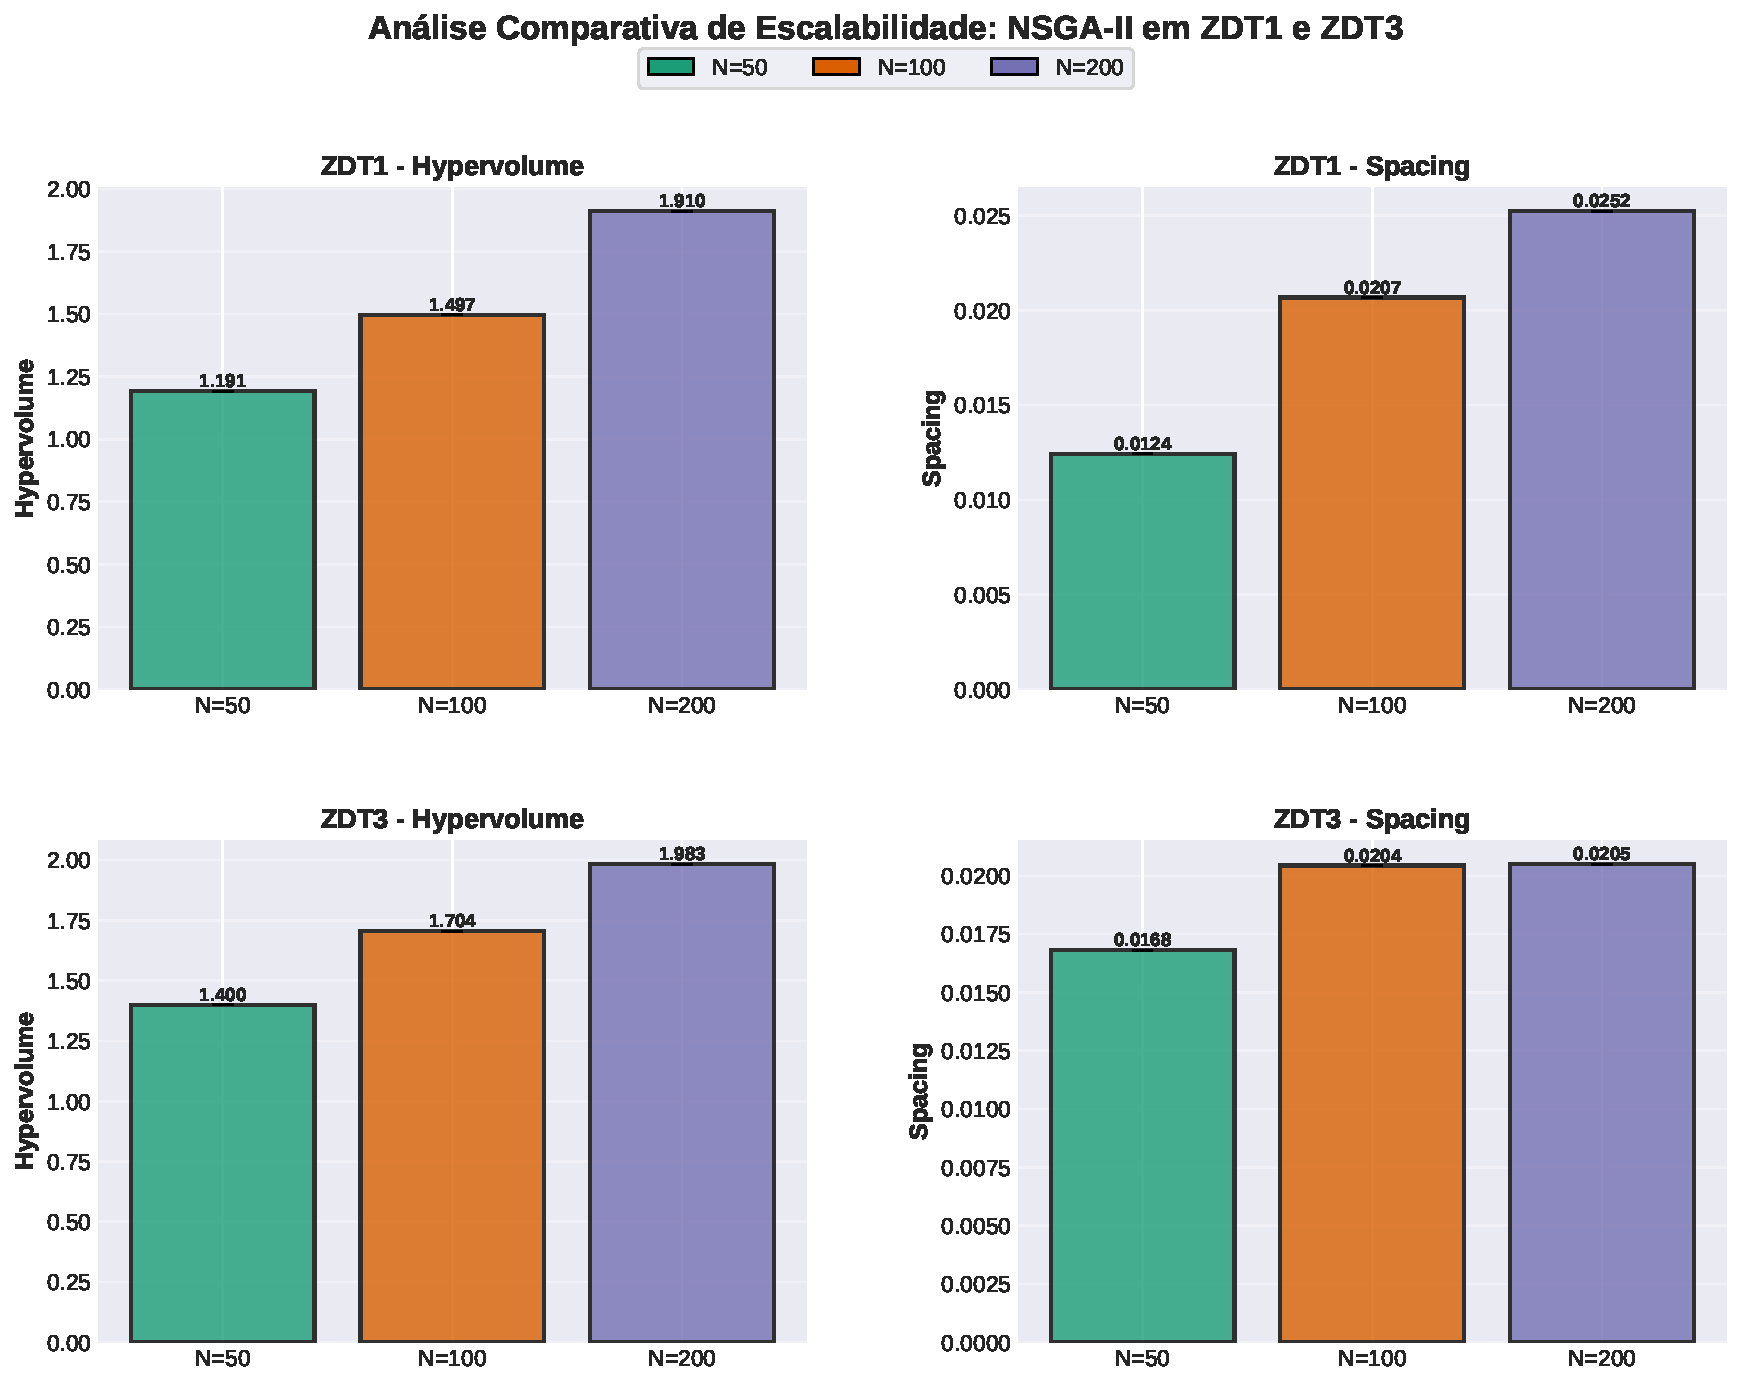
\includegraphics[width=0.95\textwidth]{../plots/K_combined_nvar_comparison.pdf}
\caption{Comparação consolidada de HV e Spacing para ZDT1 e ZDT3 em função de N. Cores indicam níveis de N (verde=50, laranja=100, roxo=200). Valores sobre barras facilitam leitura quantitativa.}
\label{fig:combined}
\end{figure}

\subsubsection{Análise Estatística de Degradação}
A Tabela \ref{tab:degradation} quantifica as taxas de degradação percentual em relação ao baseline N=50.

\begin{table}[h]
\centering
\begin{tabular}{lrrr}
\toprule
\textbf{Métrica} & \textbf{Problema} & \textbf{N=100 vs N=50} & \textbf{N=200 vs N=50} \\
\midrule
HV (degradação) & ZDT1 & -1.3\% & -3.3\% \\
HV (degradação) & ZDT3 & -1.8\% & -4.3\% \\
\midrule
Spacing (aumento) & ZDT1 & +33\% & +75\% \\
Spacing (aumento) & ZDT3 & +29\% & +65\% \\
\bottomrule
\end{tabular}
\caption{Taxas de degradação percentual das métricas. Valores negativos em HV indicam perda de qualidade; valores positivos em Spacing indicam piora na uniformidade.}
\label{tab:degradation}
\end{table}

\subsection{Interpretação Geral dos Resultados}

\textbf{Maldição da Dimensionalidade}: O aumento de N de 50 para 200 multiplica o volume do espaço de busca por $2^{150}$. Com população fixa (100), a densidade populacional cai drasticamente, explicando a degradação observada.

\textbf{Impacto Assimétrico}: HV degrada moderadamente (3-4\%), enquanto Spacing degrada severamente (65-75\%). O NSGA-II mantém convergência razoável, mas perde capacidade de distribuir soluções uniformemente.

\textbf{Diferenças entre Problemas}: ZDT3 mostra maior sensibilidade em HV (~30\% mais degradação), mas menor degradação relativa em Spacing. Hipótese: a descontinuidade força concentração nas 5 regiões, melhorando uniformidade local mas dificultando convergência global.